\paragraph{IUE03.2 Modificar identificadores} \hspace{1cm}\\ 
\label{pant:IUE03.2} 

\textbf{\textcolor[rgb]{0, 0, 0.545098}{Objetivo}}\\
Esta pantalla permite al Entrenador modificar los identificadores de una rutina.\\

\textbf{\textcolor[rgb]{0, 0, 0.545098}{Diseño}}\\
En la figura \ref{fig:IUE03.2} se muestra la pantalla \nameref{fig:IUE03.2}, por medio de la cual el Entrenador puede modificar los identificadores del elemento seleccionado.\\

En la parte inferior se encuentran los botones de Guardar y Cancelar, los cuales corresponden a guardar los cambios realizados o cancelar el registro.

\begin{figure}[H]
	\centering
		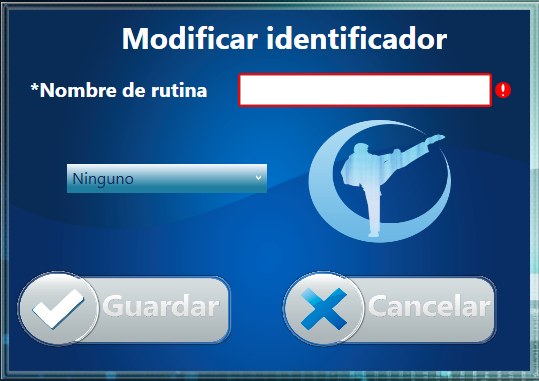
\includegraphics[scale=0.8]{./Figuras/Pantallas/IUE03_2Modificar_identificadores}
	\caption{IUE03.2 Modificar identificadores}
	\label{fig:IUE03.2}
\end{figure}

\textbf{\textcolor[rgb]{0, 0, 0.545098}{Entradas}}\\
En esta pantalla el Entrenador deberá capturar la siguiente información:

\begin{itemize}
	\item El identificador Nombre que se desea modificar.
\end{itemize}
\vspace{1em}

\textbf{\textcolor[rgb]{0, 0, 0.545098}{Controles}}
El siguiente control solo se mostrará en caso de seleccionar una rutina de entrenamiento.
\begin{itemize}
	\item \textbf{\textcolor[rgb]{0, 0, 0.545098}{Seleccionar imagen:}} Permite seleccionar al Entrenador, la nueva imagen alusiva a la rutina de entrenamiento que desea registrar.
\end{itemize}
\vspace{1em}

\textbf{\textcolor[rgb]{0, 0, 0.545098}{Comandos}}
\begin{itemize}
	\item \textbf{\textcolor[rgb]{0, 0, 0.545098}{Guardar:}} Permite al Entrenador registrar los cambios realizados a los identificadores del elemento seleccionado. 
	\item \textbf{\textcolor[rgb]{0, 0, 0.545098}{Cancelar:}} Descarta la información registrada y regresa a la pantalla \nameref{pant:IUE03}.
\end{itemize}

\vspace{1em}

\textbf{\textcolor[rgb]{0, 0, 0.545098}{Mensajes}}\\

\textbf{\nameref{msj:MSG01}}: Se muestra en la pantalla \nameref{pant:IUE03.2} cuando se modifique el identificador de manera exitosa.\\
 
\textbf{\nameref{msj:MSG12}}: Se muestra en la pantalla \nameref{pant:IUE03.2} cuando el Entrenador no haya ingresado datos a los campos obligatorios.\\

\textbf{\nameref{msj:MSG13}}: Se muestra en pantalla cuando el Entrenador haya ingresado datos con un formato incorrecto en algún campo.

\clearpage